\documentclass[]{article}

\usepackage{blindtext} % Package to generate dummy text throughout this template 

\usepackage[sc]{mathpazo} % Use the Palatino font
\usepackage[T1]{fontenc} % Use 8-bit encoding that has 256 glyphs
\linespread{1.05} % Line spacing - Palatino needs more space between lines
\usepackage{microtype} % Slightly tweak font spacing for aesthetics
\usepackage{amsmath}
\usepackage[english]{babel} % Language hyphenation and typographical rules

\usepackage{dblfloatfix} 
\usepackage{graphicx}
\graphicspath{ {./figures/} }

\usepackage[hmarginratio=1:1,top=32mm,columnsep=20pt]{geometry} % Document margins
\usepackage[hang, small,labelfont=bf,up,textfont=it,up]{caption} % Custom captions under/above floats in tables or figures
\usepackage{booktabs} % Horizontal rules in tables

\usepackage{lettrine} % The lettrine is the first enlarged letter at the beginning of the text

\usepackage{enumitem} % Customized lists
\setlist[itemize]{noitemsep} % Make itemize lists more compact

\usepackage{abstract} % Allows abstract customization
\renewcommand{\abstractnamefont}{\normalfont\bfseries} % Set the "Abstract" text to bold
\renewcommand{\abstracttextfont}{\normalfont\small\itshape} % Set the abstract itself to small italic text

\usepackage{titlesec} % Allows customization of titles
\renewcommand\thesection{\Roman{section}} % Roman numerals for the sections
\renewcommand\thesubsection{\Alph{subsection}} % roman numerals for subsections
\titleformat{\section}[block]{\large\scshape\centering}{\thesection.}{1em}{} % Change the look of the section titles
\titleformat{\subsection}[block]{\large}{\thesubsection.}{1em}{} % Change the look of the section titles

\usepackage{fancyhdr} % Headers and footers
\pagestyle{fancy} % All pages have headers and footers
\fancyhead{} % Blank out the default header
\fancyfoot{} % Blank out the default footer
\fancyhead[C]{Homework $\bullet$ June 2020 $\bullet$ Stefano F. Pitton} % Custom header text
\fancyfoot[RO, LE]{\thepage} % Custom footer text

\usepackage{titling} % Customizing the title section

\usepackage{hyperref} % For hyperlinks in the PDF

%----------------------------------------------------------------------------------------
%	TITLE SECTION
%----------------------------------------------------------------------------------------

\setlength{\droptitle}{-4\baselineskip} % Move the title up

\pretitle{\begin{center}\Huge\bfseries} % Article title formatting
\posttitle{\end{center}} % Article title closing formatting
\title{Modelling from Measurements} % Article title
\author{%
\textsc{Stefano Francesco Pitton
\thanks{PhD student Aerospace Engineering}} \\[1ex] % Your name
\normalsize Politecnico di Milano \\ % Your institution
\normalsize \href{stefanofrancesco.pitton@polimi.it}{stefanofrancesco.pitton@polimi.it} % Your email address
%\and % Uncomment if 2 authors are required, duplicate these 4 lines if more
%\textsc{Jane Smith}\thanks{Corresponding author} \\[1ex] % Second author's name
%\normalsize University of Utah \\ % Second author's institution
%\normalsize \href{mailto:jane@smith.com}{jane@smith.com} % Second author's email address
}
\date{\today} % Leave empty to omit a date
\renewcommand{\maketitlehookd}{%
\begin{abstract}
\noindent Nowadays the technology is going toward a new scientific revolution, and together with it also the matemathics, engineering, physics, computer science and almost all the other scientific and humanistic fields. This revolution is driven by the concept of Data. In this report, different strategies able to find synergy between mathematical models and available data will be described and investigate. Different dynamical problems will be considered in the following of this work in order to evaluate the capability of different data driven techniques to manage highly nonlinear system, periodic system, chaotic system and even coarse data. 
\end{abstract}
}

%----------------------------------------------------------------------------------------

\begin{document}

% Print the title
\maketitle

%----------------------------------------------------------------------------------------
%	ARTICLE CONTENTS
%----------------------------------------------------------------------------------------

\section{Introduction and Overview}

\lettrine[nindent=0em,lines=3]{I}n the era of Big Data, people are overwhelmed by an almost infinite amount of data about their personal health, the weather, the state of a building and even the motion of natural and artificial bodies in space. The availability of this vast amount of data is gradually changing the approach to solving a problem. In order to better understand the possibility and the best way to integrate data with mathematical models, different well studied problems will be considered. By working on models of which we are aware of the laws that govern its behavior it is possible to evaluate the effectiveness or not of a certain strategy, thanks to the possibility of generating artificial data through numerical simulation. 
\subsection{Lotka-Volterra Equations}
Lotka-Volterra (LV) equations are used to model the behavior of a biological system in which just two species interact, one that represents the pray and the other the predator.
\begin{equation}
\begin{aligned}
\frac{d}{dt}x &= (b - py) x \\
\frac{d}{dt}y &= (rx - d) y
\end{aligned}
\end{equation}
where $p, b, p, r$ and $d$ are nonnegative coefficients.

\subsection{Kuramoto-Sivashinsky Equation}
The Kuramoto-Sivashinsky (KS) equation represents a pattern forming system with spatio-temporal chaotic behavior. In one dimension we can write the equation as:
\begin{equation}\label{ks}
\begin{aligned}
u_t &= -uu_x - u_{xx} - u_{xxxx}  \\
&+ \textit{periodic BCs}
\end{aligned}
\end{equation}
Equation \eqref{ks} represents a nonlinear partial differential equation with chaotic  behavior. The KS equation can be used to model the diffusive instabilities in a laminar flame front.

\subsection{Lorenz Equations}
The Lorenz equations are a simplified model of convection-driven atmospheric motion. They are very sensitive to initial conditions so that a small perturbation of them causes a completely different trajectory of the system.
\begin{equation}
\begin{aligned}
x' &= \sigma (y - x) \\
y' &= rx -y - xz \\
z' &= xy -bz
\end{aligned}
\end{equation}
The trajectory of the system evolves in time generating the so-called butterfly shape.

\subsection{Belousov-Zhabotinsky Chemical Oscillator}
The Belousov-Zhabotinsky (BZ) reaction represents an example of non-equilibrium thermodynamics resulting in a nonlinear chemical oscillator. This system shows that chemical reactions do not have to be dominated by thermodynamic equilibrium and can evolve in time chaotically.

\subsection{Reaction-Diffusion}
The lambda-omega reaction-diffusion system is an example of complex spatio temporal dynamics. The system is governed by the following equations:
\begin{equation}
\begin{aligned}
u_t &= (1-(u^2 +v^2))u+ \beta (u^2 +v^2)v+d_1(u_{xx} +u_{yy}) \\
v_t &=  - \beta (u^2 +v^2)u+(1-(u^2 +v^2))v+d_2(v_{xx} +v_{yy})
\end{aligned}
\end{equation}
where the parameters $d_1, d_2$ and $\beta$ have been fixed respectively to $0.1, 0.1$ and $1$. 
%------------------------------------------------

\section{Theoretical Background}
In this paper we will consider nonlinear dynamical systems of the form:
\begin{equation}\label{dynsys1}
    \frac{d}{dt}\textbf{x} =\textbf{f}(\textbf{x}(t), \boldsymbol\beta)
\end{equation}
where $\textbf{x}(t) \in \mathcal{R}^n$ denotes the state of the system at time t, $\boldsymbol\beta$ denotes the system parameters and $\textbf{f}$ describes the evolution of the system in time.
In the context of a data-driven approach, we have to consider that we don't have the differential equations that govern the system but just some realizations of it. We can describe the relationship between two consecutive realizations as a discrete-time dynamical system:
\begin{equation}\label{dynsys2}
    \textbf{x}_{k+1} =\textbf{F}(\textbf{x}_k)
\end{equation}
where each realization is interpreted as a sample on the system trajectory.
%
\subsection{Dynamic Mode Decomposition}
DMD is a powerful tool that can be applied in the analysis of a dynamical system. The idea behind this algorithm is that it is possible to express the future state as a linear combination of the actual state. At the core of DMD, there is the Singular Value Decomposition (SVD), an algorithm that allows discovering the principal directions of the data set. These principal directions are extremely useful since allow for a linear transformation of the coordinate system into one in which we can exploit the variance of the features and we can apply dimensionality reduction.\\
The DMD algorithm allows to discover the best representation in term of reduced spatial coordinates and a way in which advance this coordinates in time \cite{brunton2019}. Given $m$ realizations, or snapshots, of an $n-$dimensional state vector $\textbf x$ we can stack them into an $n \times m$ matrix $\textbf X$. From the matrix $\textbf X$ we can build another matrix $\textbf X'$, which is nothing but the former matrix shifted one time step ahead. The goal is to discover the best fit linear operator that allows to advance the state vector in time:
\begin{equation}\label{bestfit}
    \textbf{X'} \approx \textbf{A} \textbf{X}
\end{equation}
The $\approx$ symbol is used since in a general framework, the state matrices can be non-square. The best fit linear operator can be computed as:
\begin{equation}\label{bestfit}
    \textbf{A} = argmin \parallel \textbf{X'} - \textbf{A} \textbf{X} \parallel_F = \textbf{X'} \textbf{X}^\dagger 
\end{equation}
where $\parallel \parallel_F$ denotes the Frobenius norm and $^\dagger$ denotes the pseudo-inverse. The most efficient way to solve this problem, especially in case of high dimensional state matrix, is computing the spectral decomposition of the pseudo-inverse through the economy SVD:
\begin{equation}\label{svd}
    \textbf{X} \approx \tilde{\textbf{U}} \tilde{\bf\Sigma} \tilde{\textbf{V}}^*
\end{equation}
where the $\tilde{}$ indicates that the economy SVD with rank $r$ has been used, $^*$ denotes the complex conjugate transpose and $\tilde{\textbf{U}} \in \mathcal{C}^{n \times r}$, $\tilde{\textbf{V}} \in \mathcal{C}^{m \times r}$, and $\tilde{\bf{\Sigma}} \in \mathcal{C}^{r \times r}$. Note that, $r$ can be the rank of the original matrix $\textbf X$ or smaller value used to embed the data set into a lower dimension. At this point we can project the matrix $\textbf{A}$ onto the $\tilde{\textbf{U}}$ modes:
\begin{equation}\label{atilde}
    \textbf{A} = \tilde{\textbf{U}}^* \tilde{\textbf{A}} \tilde{\textbf{U}} = \tilde{\textbf{U}}^* \textbf{X'} \tilde{\textbf{V}} \tilde{\bf{\Sigma}}^{-1}
\end{equation}
Since we reduce reduce the dimensionality of $\textbf{A}$ through a similarity transformation, the non zero eigenvalues have been preserved The spectral decomposition of $\tilde{\textbf{A}}$ can be computed as:
\begin{equation}\label{specdec}
    \tilde{\textbf{A}} \textbf{W} = \textbf{W} \bf{\Lambda} 
\end{equation}
where the diagonal matrix $\bf{\Delta}$ contains the DMD eigenvalues, equal to the eigenvalues of the matrix $\textbf A$. The DMD modes, which correspond to the high dimensional modes of the matrix $\textbf A$, can be computed as:
\begin{equation}\label{specdec}
    \bf{\Phi} = \textbf{X'} \tilde{\textbf{V}} \tilde{\bf{\Sigma}}^{-1} \textbf{W}
\end{equation}
Given the DMD modes $\bf{\Phi}$ and the DMD eigenvalues $\bf{\Lambda}$ we can compute the state vector in any time instant as:
\begin{equation}
    \textbf{x}_k = \bf{\Phi}\bf{\Lambda}^{k-1} \textbf{b} 
\end{equation}
where the mode amplitudes are computed given the initial conditions as $\textbf{b} = \bf{\Phi}^\dagger\textbf{x}_1$. 

\subsection{Time-delay Embedding}
The main idea behind DMD is the capability to approximate the dynamics of the system as a linear combination of the state vector. This idea is the same as when applying linear regression, in which a linear relationship between the input features and output is assumed. We are not living in a linear world and it is very difficult that this assumption holds strictly. The main advantage of building a linear model is the possibility to interpret the results and apply control laws but, we need to be able to manage situations in which this simple idea cannot be applied directly. The simplest case to consider is the one in which we are not able to measure directly the entire states of the system, in this situation, there could be latent variables that influence the dynamics but that we can't directly see. For this reason, latent variables, are sometimes also called hidden variables. One possibility to overcome this situation is to project the state vector into a higher dimension and build a linear model into this new space. This approach is very popular in the machine learning community, just think about support vector machine or linear regression into an extended feature space. In the context of DMD, this idea is also at the core of the \textit{Koopman} operator, finding the best coordinate system in which express our model as a linear one. A very intuitive approach to manage situations in which linear combinations of our state space vector is not enough is one of \textit{time-delay embedding}. In time-delay embedding, we increase the state space by stacking together different delayed copies of the vector $\textbf x$. To better understand how to build the matrix $\textbf X$, let's consider the case of a k time-delay embedding. The resulting matrix, called the \textit{Hankel} matrix, will be composed as:
\begin{equation}
\textbf{H} = 
    \begin{bmatrix}
        x(t_0) & x(t_1) & \dots &  x(t_M)\\
        x(t_1) & x(t_2) & \dots &  x(t_{M+1})\\
        \vdots &  \vdots & \ddots &  \vdots \\
        x(t_k) & x(t_{k+1}) & \dots &  x(t_{M+k}) 
    \end{bmatrix}
\end{equation}
where here we use $M$ columns instead of $m$ since, due to the time delay, we can't use the entire state history in each row. Applying SVD to $\textbf{H}$ we can gain more insight into the real rank of the system, discovering the effective number of the latent variables through the shadow of the manifold in which the system leaves. The real rank of the system is obtained by looking at the energy contained, or variance explained, by each of the singular values.

\subsection{Regression}
The goal of a regression problem is to learn a mapping from a given $n$-dimensional vector $\textbf{x}$ of input variables to one or more continuous target variables $\textbf{y}$ \cite{bishop2006}. Some examples of regression problems are the prediction of a stock market price, the prediction of future emissions of CO$_2$, the effect of an actuation in robotics and so on. A general regression problem can be formulated as:
\begin{equation}\label{regression}
y(\textbf{x}, \textbf{w}) = w_0 + \sum_{j=1}^{n-1}w_j x_j = \textbf{w}^T\textbf{x}
\end{equation}
Our goal is to find the best values of the weights $\textbf{w}$. Different approaches exist to find the best combination of weights and the most common are based on the minimization of a loss function.
\begin{equation}\label{loss}
\mathcal{L}(\textbf{w})  = \mathcal{L}_D(\textbf{w}) + \lambda \mathcal{L}_w(\textbf{w})
\end{equation}
In equation \eqref{loss} the loss function is composed by two terms: the first one is a measure of the fit quality, typically the squared loss error, and the second one is a term introduced to avoid to overfit the data. According to the second term of the loss we can have: standard Least Squares with $\mathcal{L}_w = 0$, Ridge regression with $\mathcal{L}_w = \parallel \textbf{w} \parallel_2^2$ , Lasso regression with $\mathcal{L}_w =\parallel \textbf{w} \parallel_1$ or Elastic Net which is a combination of Lasso and Ridge. The parameter $\lambda$ determines the intensity of the regularization and is a parameter to be choose with cross-validation.
\subsection{Sparse Identification of  Nonlinear Dynamics (SINDy)}
An important observation of most physical system is that their dynamics is usually characterized by few parameters, making the equations sparse in the high-dimensional function space. This is also the main idea behind the Lasso algorithm where among the infinite solutions to the linear problem, the one with the most zero weights is favoured. In the SINDy approach, the philosophy is the same but, with a different point of view. Differently from the classical application of regression in machine learning, where the interest is just in fitting the data, without any distinction between a dynamics or static system, in SINDy we try to explicitly discover the coefficient of the dynamic map in \eqref{dynsys2}. Given a state matrix $\textbf{X}$ and its derivative $\dot{\textbf{X}}$:
\begin{equation}
\textbf{X} = 
\begin{bmatrix}
	x_1(t_0) & x_2(t_0) & \dots &  x_n(t_0)\\
	x_1(t_1) & x_2(t_1) & \dots &  x_n(t_1)\\
	\vdots &  \vdots & \ddots &  \vdots \\
	x_1(t_m) & x_2(t_m) & \dots &  x_n(t_m) 
	\end{bmatrix} 
	\quad
	\dot{\textbf{X}} = 
	\begin{bmatrix}
	\dot x_1(t_0) & \dot x_2(t_0) & \dots &  \dot x_n(t_0)\\
	\dot x_1(t_1) & \dot x_2(t_1) & \dots &  \dot x_n(t_1)\\
	\vdots &  \vdots & \ddots &  \vdots \\
	\dot x_1(t_m) & \dot x_2(t_m) & \dots &  \dot x_n(t_m) 
\end{bmatrix}
\end{equation}
Next we build a library of possible linear and  nonlinear transformation of the state matrix:
\begin{equation}
\bf{\Theta}(\textbf{X}) = 
\begin{bmatrix}
\vline & \vline & \vline &  &  \vline & \vline & \\
\textbf{1} & \textbf{X} & \textbf{X}^2 & \dots & sin(\textbf{X}) & cos(\textbf{X}) & \dots \\
\vline & \vline & \vline &  & \vline & \vline & 
\end{bmatrix}
\end{equation}
At this point we can set the sparse regression problem as determine the sparse vectors of coefficients $\bf\Xi = [\boldsymbol\xi_1, \boldsymbol\xi_2, ..., \boldsymbol\xi_n]$ that determine which nonlinearity is active:

%------------------------------------------------
\begin{equation}
\dot{\textbf X} = \bf \Theta(\textbf X) \bf{\Xi}
\end{equation}
\section{Algorithm Implementation and Development}
All the algorithms applied to this work have been written in Python 3.7 and through the use of Jupiter and Colab notebooks. Several libraries have been involved:

\begin{itemize}
    \item \textit{NumPy}: linear algebra library,
    \item \textit{SciPy}: efficient numerical routines library,
    \item \textit{Matplotlib}: visualization library,
    \item \textit{Scikit-learn}: predictive data analysis library,
    \item \textit{PyTorch}: machine learning and deep learning library,
    \item \textit{pyrenn}: neural network library
\end{itemize}

The use of these libraries, instead of hard code coding, has allowed faster programming and more time for experimentation.
%------------------------------------------------

\section{Computational Results}
In this section, all the most relevant results will be briefly presented and discussed.

\subsection{Analysis of Population Dynamics}
\subsubsection{DMD}
The first step in the analysis of the dynamics of the snowshow hare and Canada lynx populations has been the augmentation of the data set. Due to the small real data available a cubic spline has been applied to move from $30$ to $581$ samples. The use of splines leads to population values lower than zero, obviously impossible in nature. Has been found that substituting all the population values lower than zero with $1$ help to obtain better results in the dynamics discovery. The first strategy adopted was to approximate and discover the linear model by DMD. In Figure \ref{fig:fig1} the real dynamics and the one approximated through DMD have been reported.
\begin{figure}[!t]
\centering
\includegraphics[width=0.9\textwidth]{../figures/dmd.pdf}
\caption{Real data (left) and DMD approximation (right). Due to the complex behavior exhibited by the two population as simple linear model fails to capture the dynamics.}
\label{fig:fig1}
\end{figure}
Can be easily seen that a simple DMD model onto a $2 \times 580$ matrix is not sophisticated enough to capture the dynamics of the system. Nevertheless, the simple DMD model has discovered that the lynx population increases just after an increase in the hare population, and decreases in the same manner. This is a typical behavior of a predator-pray system. The model can be refined by the adoption of an Hankel matrix through the time-delay embedding method. In the specific, $4$ different time delay have been considered: $10, 50, 100$ and a full embedding provided by the \textit{hankel} method provided by the scipy library. In the full embedding, if the state vector has $m$ time samples, it produces $m$ time-delayed embeddings padding with zeros the last position of each new row added to the matrix in order to compensate the time shift. The real rank of the system can be discovered by looking at the energy captured by the singular values obtained by the SVD of the Hankel matrix. From the Figure \ref{fig:fig2} we can see that, by increasing the time-delay more singular values pop-up from the zero value. The more the non-zero singular values, the more the hidden variables that are not present in the data set but that contribute to the system dynamics. Successively, the DMD has been applied to the four Hankel matrices with ranks respectively, $4$, $10$, $20$ and $40$.
\begin{figure}[!t]
\centering
\includegraphics[width=0.9\textwidth]{../figures/td_energy.pdf}
\caption{Energy accounted for by the singular values of the 4 different Hankel matrix. Increasing the time-delay embedding increase the rank of the embedding manifold.}
\label{fig:fig2}
\end{figure}
At this point is important to point out that, our goal is not just the mere approximation of the data points but, the goal is to approximate the underlying model, in such a way to be able to forecast unseen future times. To this end, the available points are partitioned into training points and testing points. Since we want to forecast and not interpolate, the training set is composed by the first $80\%$ points, according to the time axis, and the testing points are the remaining ones. Differently, using random split to generate the two data set the result will be just an interpolation, without the possibility to evaluate the effective capacity of the model. Below, in Figure \ref{fig:fig3} the approximated behaviors are reported.
\begin{figure}[!t]
\centering
\includegraphics[width=0.9\textwidth]{../figures/td_dmd.pdf}
\caption{Approximation of the system dynamics via DMD. The real behavior has been reported with almost transparent lines. The gray boxes cover the states used to train the models}
\label{fig:fig3}
\end{figure}
We can see that by increasing the time-delay embedding, and consequently the latent variables introduced into the model, the DMD expansion becomes more capable of follow the real system. Due to the high nonlinear nature of the system, the forecasting is really difficult, the models with $100$ and full embeddings can qualitatively follow the real behavior but not quantitatively. 
\subsubsection{Regression Model}
In the previous paragraph two completely data driven methods have been considered. In mathematics, the analysis of a biological system comprising pray and predator can be performed with the Lotka-Volterra (LV) differential equations. Here we want to apply regression to fit the data to the parameters of LV equations. Ordinary least squares linear regression,  Ridge and standard pseudo-inverse have been applied to the data. As did previously, the data has been splitted in $80\%$ training and $20\%$ test. The best approximation of the system dynamics has been found with the pseudo inverse, but, the really low $R^2=-2.9$ makes this model really unreliable. In Figure \ref{fig:fig4} the true behavior and the one obtained by integrating the LV model with fitted parameters to data is reported. Except for the delayed picks of the predator with respect to the pray, the model is completely unable to represent the system dynamics.
\begin{figure}[!t]
	\centering
	\includegraphics[width=0.9\textwidth]{../figures/history_fit.pdf}
	\caption{Real behavior of the system (left) and approximation via integration of LV equations with fitted parameters (right). The gray boxes cover the states used to train the model}
	\label{fig:fig4}
\end{figure}
\subsubsection{Best Fit Nonlinear Sparse Model}
Another possibility to approximate the system dynamics is through sparse identification of the best fit nonlinear model. A library of candidate feature expansion was built and the Lasso algorithm has been applied to discover which of the features affect the system behavior. Once discovered the sparse parametrization of the dynamics the envelope of the species in time can be reconstructed as:
\begin{equation}\label{nlbestfit}
\textbf{x}(t+1) = \text{LassoModel}_{\alpha_{opt}}(\textbf{x}(t)) \Delta t + \textbf{x}
\end{equation}
where the Lasso model was trained to approximate the relation between $\textbf{x}$ and $d/dt \textbf{x}(t)$. The Lasso algorithm has been trained with different shrinkage coefficient and the choice of the best was made by valuating the $r^2$ error between the reconstructed dynamics and the real one. In Figure \ref{fig:fig5} can be observed the library involved and the value of the coefficient for the best Lasso model with $\alpha=0.005$.
\begin{figure}[!b]
	\centering
	\includegraphics[width=0.9\textwidth]{../figures/nl_param_fit.pdf}
	\caption{Sparse coefficients of the best fit nonlinear model}
	\label{fig:fig5}
\end{figure}
The approximation of the dynamics is reported in Figure \ref{fig:fig6}
\begin{figure}[!t]
	\centering
	\includegraphics[width=0.9\textwidth]{../figures/nl_history_fit.pdf}
	\caption{Real behavior of the model (left) and reconstruction of the dynamics with SINDy algorithm (right). The gray box covers the states used to train the model}
	\label{fig:fig6}
\end{figure}
Also in this case the dynamics of the two species is not captured well, indeed the model just predict the means as confirmed by the $R^2$ equal to $0$.
%------------------------------------------------
\subsection{Analysis of Kuramoto-Sivashinsky and Reaction-Diffusion Equations}
\subsubsection{Time-Marching Neural Network}
The behavior of the KS equation has been analyzed and an ANN has been built to approximate the Runge-Kutta methods for the simulation of the system dynamics. The approximation of the Runge-Kutta methods has been obtained by training a network able to predict the future state given the actual one in such a way to advance the system in time. First of all a time-spatial data set composed by $n_x=128$ points in space and $n_t=251$ points in time has been built. Successively, this data set has been splitted into train test sets according to the proportion $ 80/20$. Since we want to be able to forecast the system dynamics the data set split has been made in such a way that the training set is the first part the time history and the test one, the last part. Four different NN have been considered with a fixed architecture but a different number of neurons in each layer. The hidden layers are 3, all with ReLU activation functions while for the output layer no activation functions are used (i.e. identity transfer function). No regularization like weights decay or dropout have been considered. The NN considered are composed respectively by $n_x/2$, $n_x$, $2n_x$ and $3n_x$ hidden units and were trained for $1000$ epochs. In Figure \ref{fig:fig7} the difference between the real behavior and the ones approximated by the ANN are reported, accompanied by the relative Mean Squared Errors in \ref{table:1}.
\begin{figure}[!t]
	\centering
	\includegraphics[width=0.9\textwidth]{../figures/fore_err.pdf}
	\caption{Real behavior of the model (left) and reconstruction of the dynamics with SINDy algorithm (right). The gray box covers the states used to train the model}
	\label{fig:fig7}
\end{figure}
\begin{table}[!b]
	\begin{centering}
	\begin{tabular}{cccc}
		\hline
		\multicolumn{4}{c}{MSE}       \\ \hline
		ANN 1 & ANN 2 & ANN 3 & ANN 4 \\ \hline
		1.65  & 1.29  & 1.18  & 1.16  \\ \hline
	\end{tabular}
\caption{Mean squared errors of the $4$ different ANNs}
\label{table:1}
\end{centering}
\end{table}
We can see that the network $4$ is the one that achieves the best performance onto the test set. However, must be pointed out that, this is the result for the specific training considered so it is not true that the ANN $4$ is always the best. From this time this trained model will be used for the following analysis. In Figure \ref{fig:fig8} the forecasting of the network until the final time of $200s$ is reported.
\begin{figure}[!t]
	\centering
	\includegraphics[width=0.9\textwidth]{../figures/fore.pdf}
	\caption{Forecasting of ANN 3 for $200 s$ (right) versus integration of the differential KS equation (left)}
	\label{fig:fig8}
\end{figure}
We can see that the network start to reproduce some kin of periodic patterns, being unable to follow the chaotic behavior of the system.
\subsubsection{Different Initial Conditions}
At this point we evaluate  if the ANN is able to generalize also to different initial conditions of the ones used to generate the training data. First of all we try the previous trained ANN with a different parameter L, governing the shape of the initial conditions. The L value is changed from $32$ to $34$ and what is observed is that the network does not capture this modification and still behaves as in the case of L equal to $32$. After this tentative the same ANN 4 has been retrained with a data set composed by simulations with $L = 2, 4, 12, 16, 20, 27, 32, 45, 55$ and $64$ for $2000$ epochs and adding as input also the actual L. Also in this case there were very low performances, and reason is probably in the highly nonlinear and chaotic behavior of the system which produces completely different dynamical patterns also for very small changes in the initial conditions. Just to have an idea of how bad the network si behaving after being trained with a data set composed of time history of a so chaotic system, in Figure \ref{fig:fig9} the result of the time-marching ANN is reported.
\begin{figure}[!t]
	\centering
	\includegraphics[width=0.9\textwidth]{../figures/fore_diff_ic2.pdf}
	\caption{Real behavior (left) and approximation through time-marching neural network}
	\label{fig:fig9}
\end{figure}
\newpage
\subsubsection{Analysis of Reaction Diffusion System}
In this section will be made a brief description of the application of a neural network to the approximation of the RD system. A data set composed by $201$ snapshots of the $32 \times 32$ spatial discretization of the RD system have been generated with Runge-Kutta integration scheme. The standard SVD has been applied to the flattened state matrix composed by the first $200$ snapshots in order to compute a lower dimension representation of the matrix. The rank of the reduction has been chosen by looking at the energy captured by each mode, and in the specific case a rank $14$ has been considered. In this way the original spatial dimension of $32 \times 32$ has been drastically reduced making easier to train a neural network to forecast the future state of the system. A $3$ hidden unit architecture, with ReLU activation function and $100$ nodes for layer has been trained with the training set composed by the first $161$ time samples. This network, has been successively applied recursively, to predict the future states starting from the last time snapshot used in the training set. It is possible to see that the network is capable to capture the behavior of the system for few time step ahead from the training set in Figure \ref{fig:fig10} but, accumulating errors during the forecast for long time step ahead is not accurate enough Figure \ref{fig:fig11}.
\begin{figure}[!b]
	\centering
	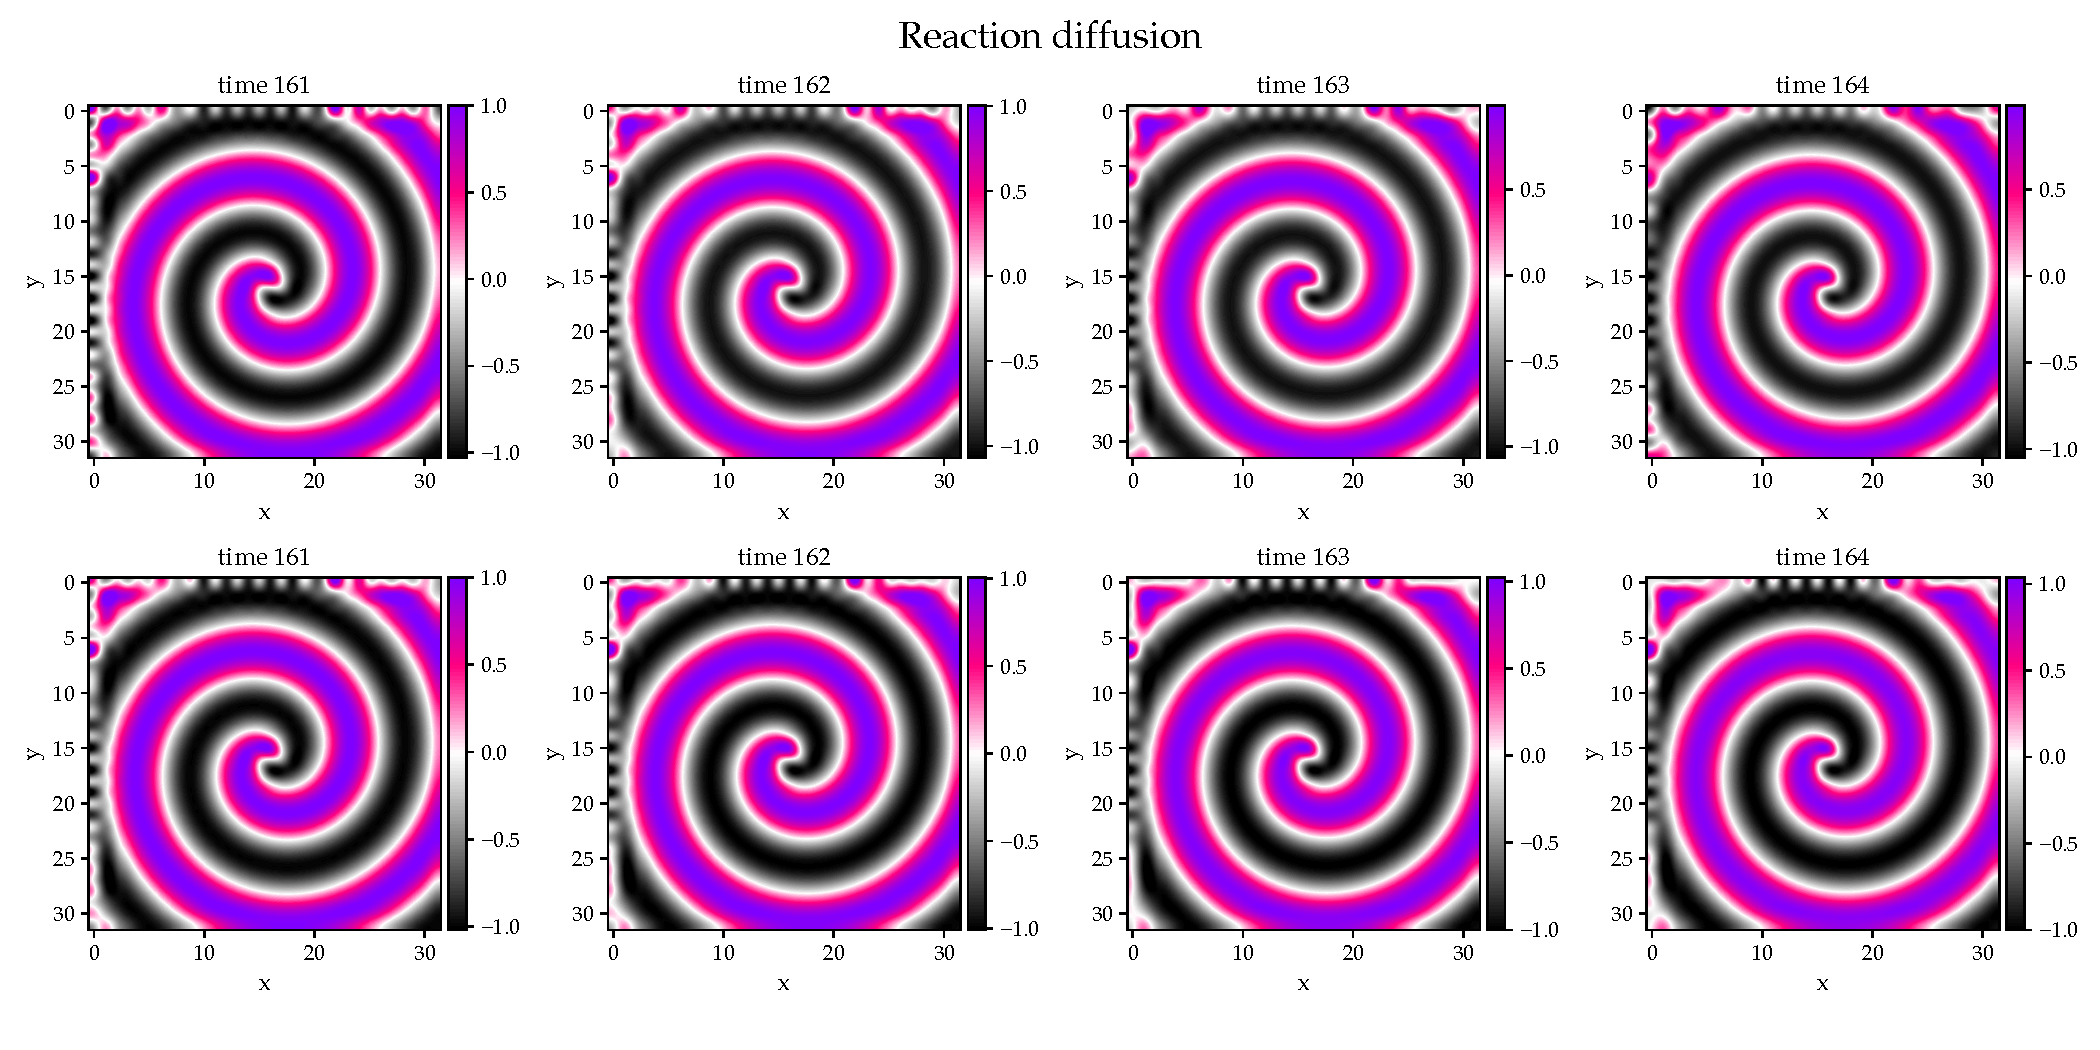
\includegraphics[width=0.9\textwidth]{../figures/forecast_RD.pdf}
	\caption{Upper row real behavior, lower row prediction obtained by applying recursively the ANN near in future}
	\label{fig:fig10}
\end{figure}
\begin{figure}[!t]
	\centering
	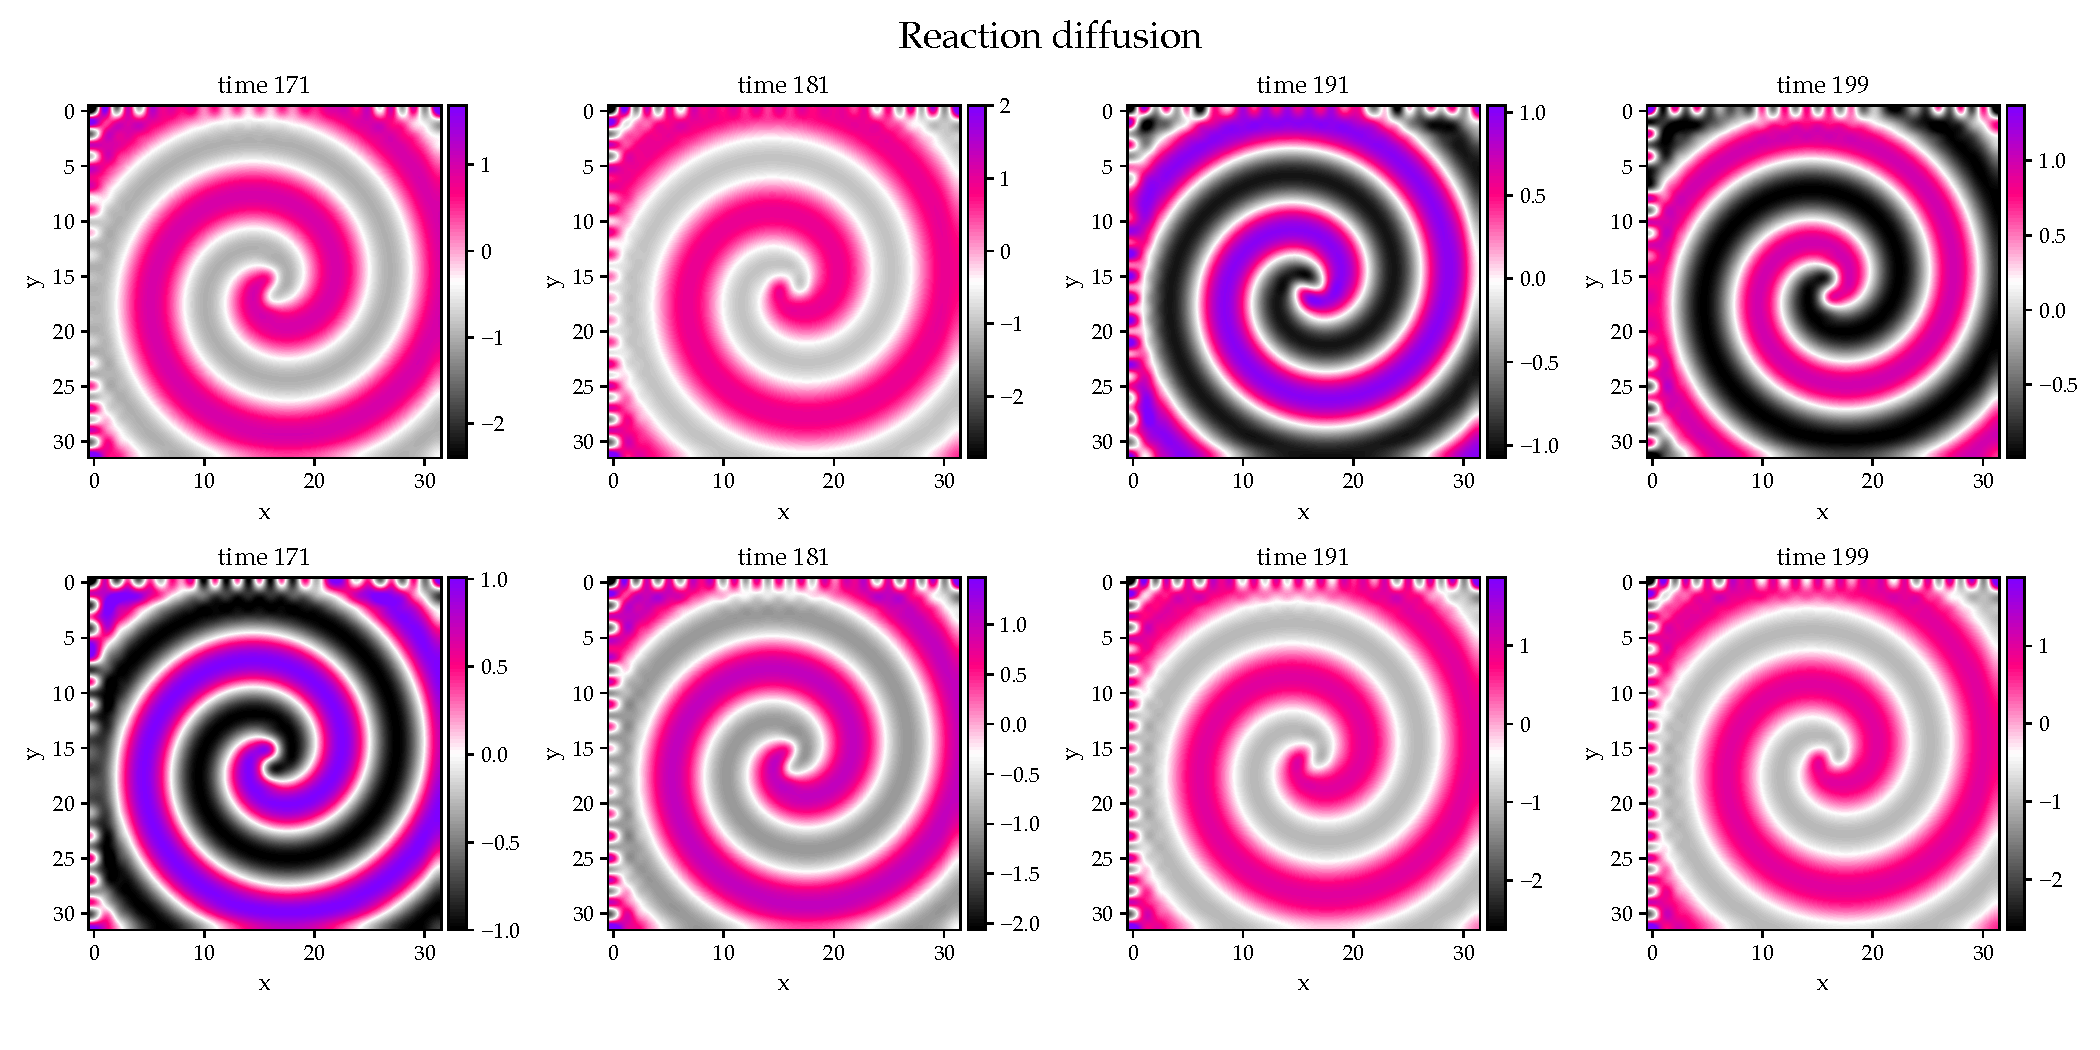
\includegraphics[width=0.9\textwidth]{../figures/forecast_RD2.pdf}
	\caption{Upper row real behavior, lower row prediction obtained by applying recursively the ANN far in future}
	\label{fig:fig11}
\end{figure}
\begin{figure}[!t]
	\centering
	\includegraphics[width=0.9\textwidth]{../figures/comparison_train.pdf}
	\caption{Real and approximated history of the $x(t)$ coordinate of Lorenz equations. On the left the results of the ANN trained with LM and on the right those of the ANN trained with Adam}
	\label{fig:fig12}
\end{figure}
\subsection{Analysis of Lorenz Equations}
\subsubsection{Neural Network Approximation}
In this section will be presented the results on the use of a neural network to approximate the dynamics of Lorenz's equations. Two different type of architectures has been trained, one exploiting the PyTorch library with $3$ hidden units, $10$ neurons for layer, \textit{ReLU} activation function and trained with SGD, and the other exploting the pyrenn library, with same architecture but \textit{tanh} activation functions and trained with Levenberg–Marquardt. In Figure \ref{fig:fig12} the envelope for the $x$ coordinate of the Lorenz equations for different values of $\rho$ have been reported. 
The ANN trained with Levenberg–Marquardt (LM) completely outperform the ANN trained with SGD. This result is probably due to the fact the SGD is a powerful, and probably the only algorithm, that can be applied in case of Big Data but for simple problems, in terms of input dimension, the possibility to approximate the Hessian matrix helps improving the training. On the other hand, the approximation of the Hessian makes the training really slow when the dimension of the input space or of the hidden layers become high. Should be observed that was not applied the standard SGD algorithm but a more sophisticated version called Adam. Afterwards, the network trained with LM has been applied to the Lorenz equations with $\rho$ values never seen during the training. In Figure \ref{fig:fig13} it is possible to see that the model works quite well also on out-of-sample parameterizations.
\begin{figure}[!b]
	\centering
	\includegraphics[width=0.9\textwidth]{../figures/rho_oos.pdf}
	\caption{ANN trained with LM algorithm performance onto unseen dynamics. The different dynamics have been generated integrating the Lorenz equations with different values of $\rho$}
	\label{fig:fig13}
\end{figure}
\subsection{Analysis of  Belousov-Zhabotinsky Chemical Oscillator Movie}
The video of the BZ oscillator has been analyzed with the goal of finding its principal modes. First of all the singular values energy has been calculated in order to decide the rank-truncation of the system for the DMD expansion. With a rank truncation of $101$ nice results have been obtained. As in the previous problems the available data has been split in train and test and, in Figure \ref{fig:fig14} the DMD approximation of the first time instants are reported, they were in training set and a good approximation has been achieved. In Figure \ref{fig:fig15}, it is possible to see that good approximations are obtained also for the frames in the test set. In this case the DMD modes fails to capture the behavior of the system in the top right of the pictures, where new wave ridges begin to appear at high frequency.
\begin{figure}[h]
	\centering
	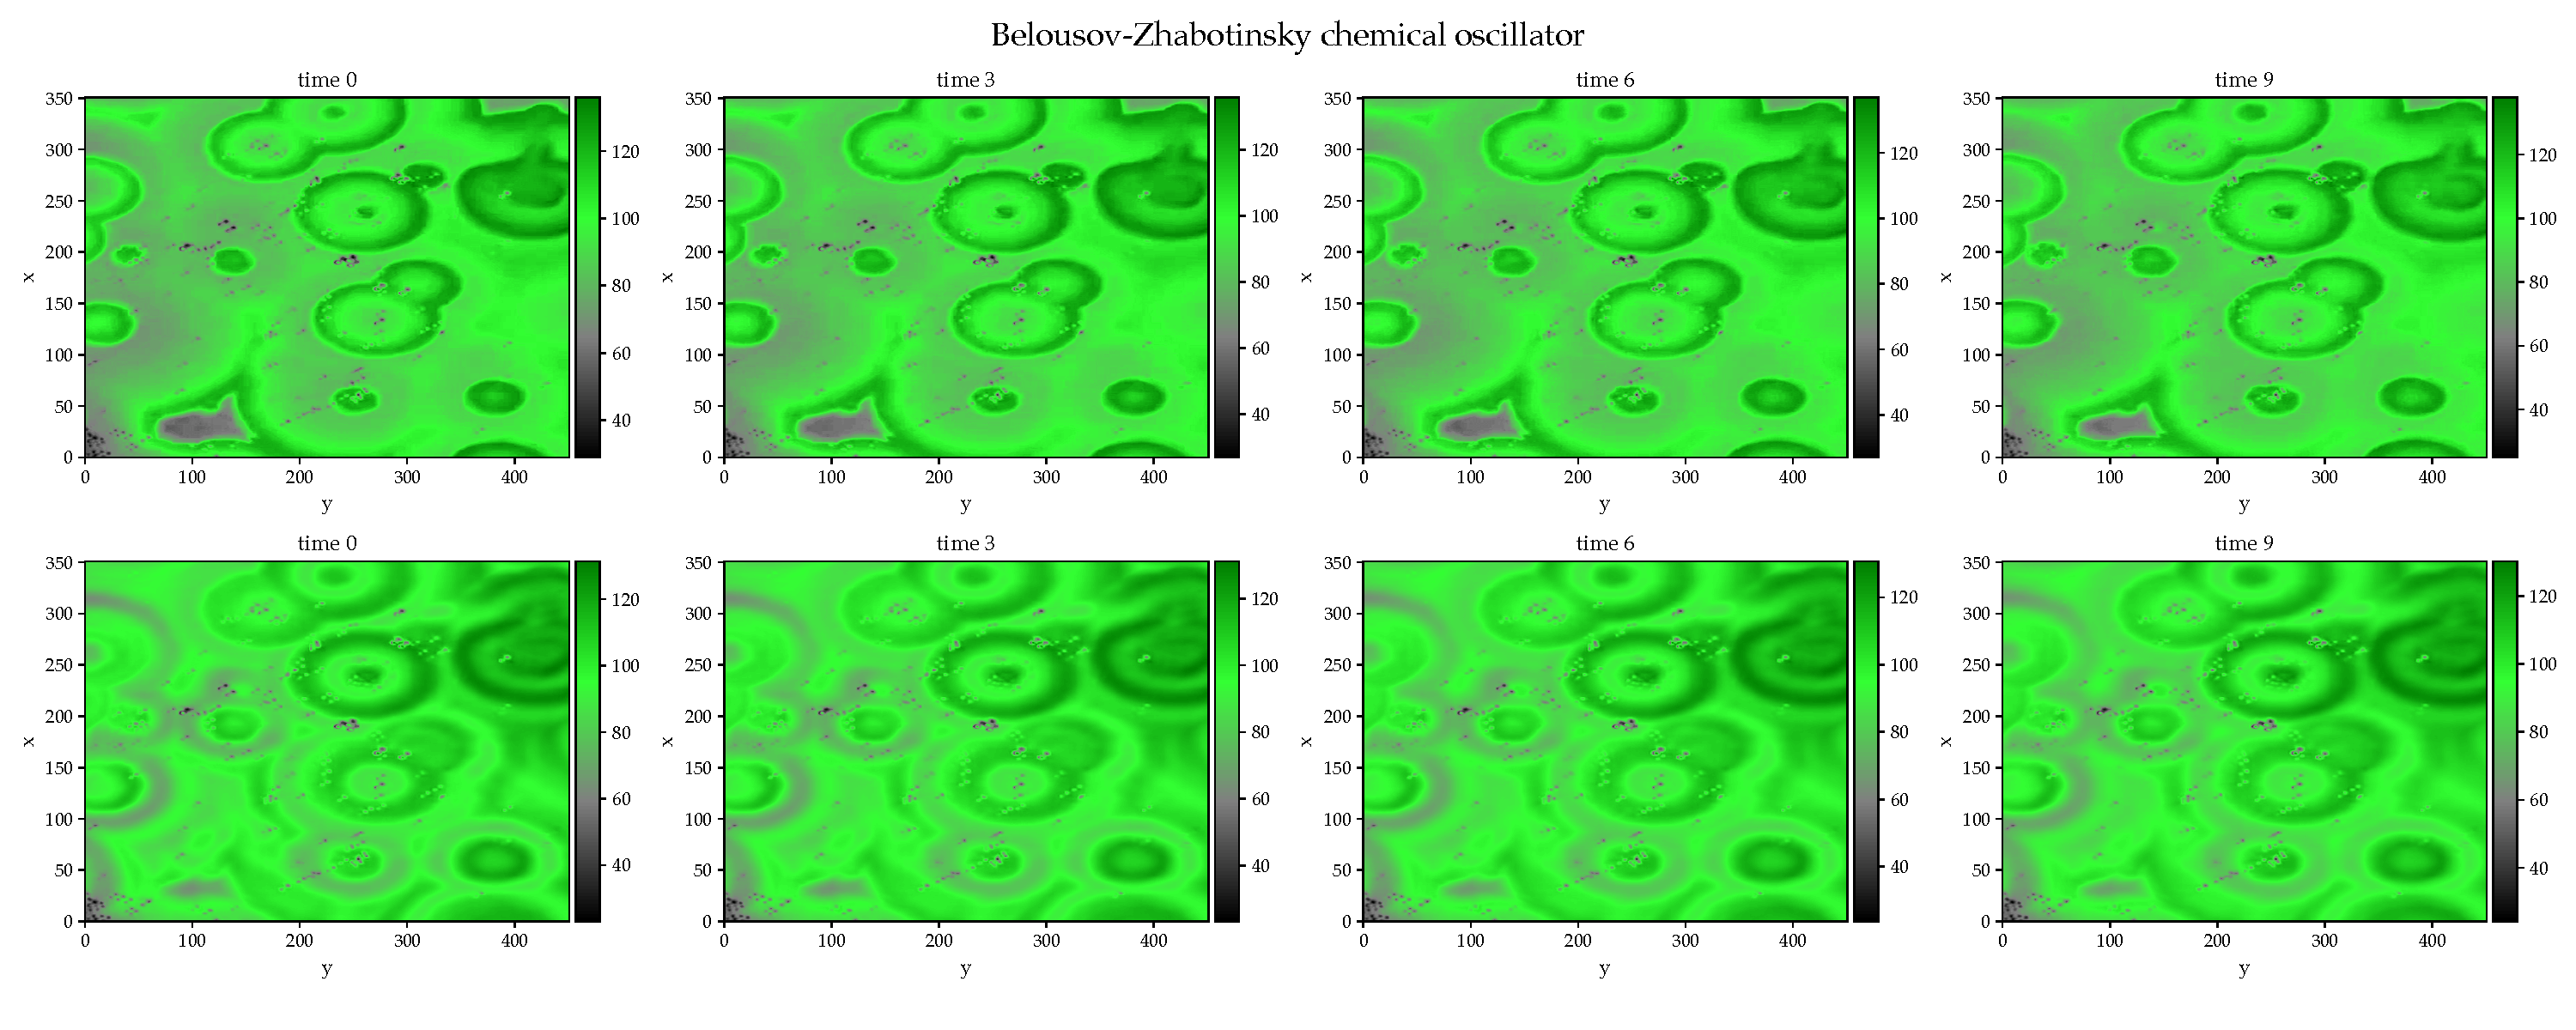
\includegraphics[width=0.9\textwidth]{../figures/BZ_closetime.pdf}
	\caption{DMD approximation on the training data set}
	\label{fig:fig14}
\end{figure}
\begin{figure}[h]
	\centering
	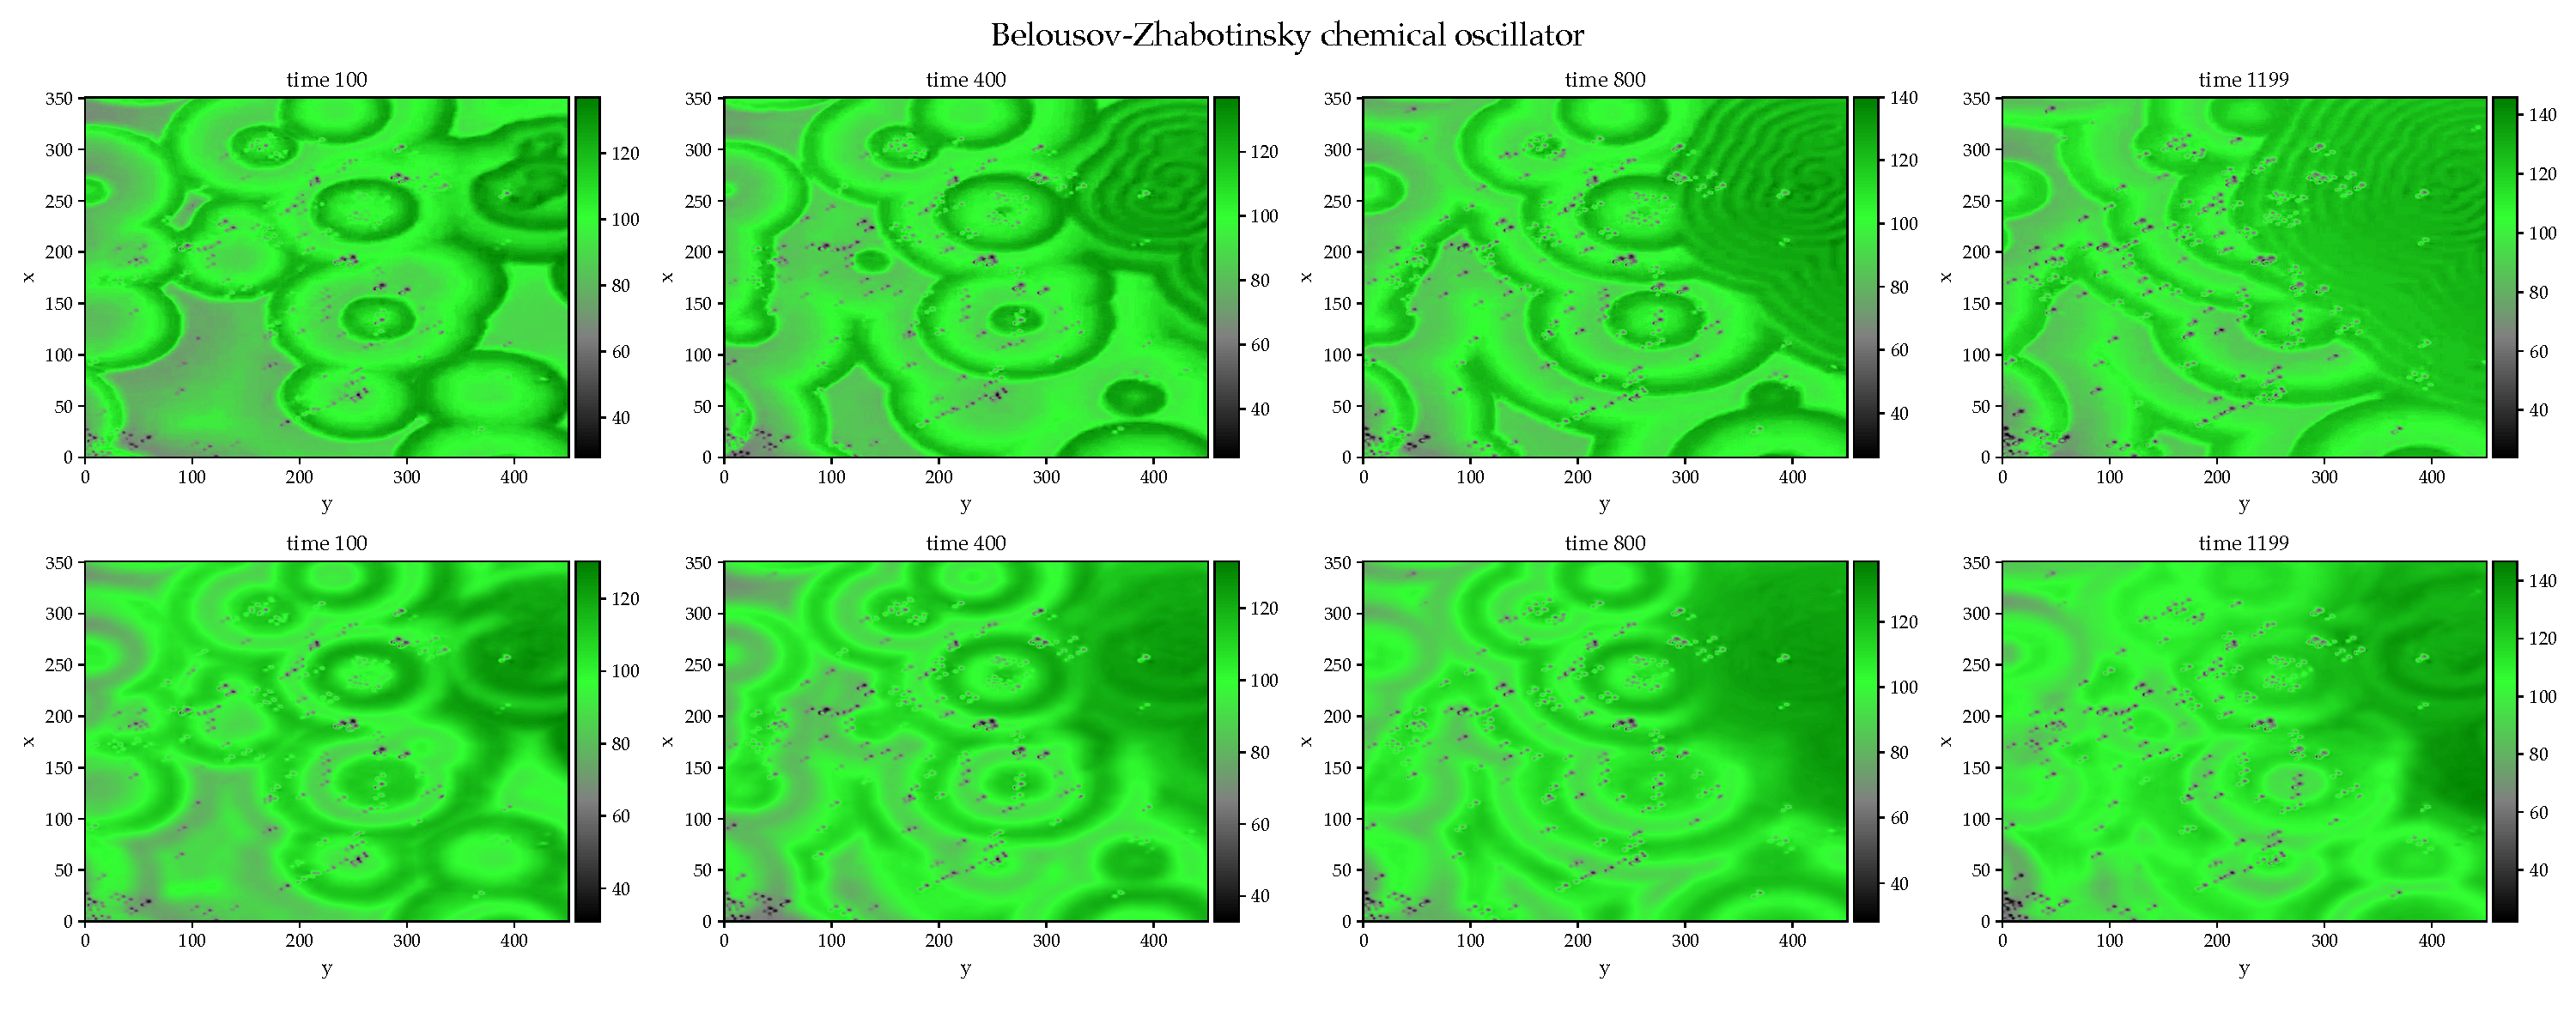
\includegraphics[width=0.9\textwidth]{../figures/BZ_fartime.pdf}
	\caption{DMD approximation on the test data set. This is a forecasting since the test set are the last frames of the video}
	\label{fig:fig15}
\end{figure}
It is also interesting to look at the reduced left and right singular vectors. The first $4$ singular vectors are reported in Figure \ref{fig:fig16}. Surprisingly enough, the first spatial mode does not reflect the concentric structures but the bubbles developed during the reaction.
\begin{figure}[h]
	\centering
	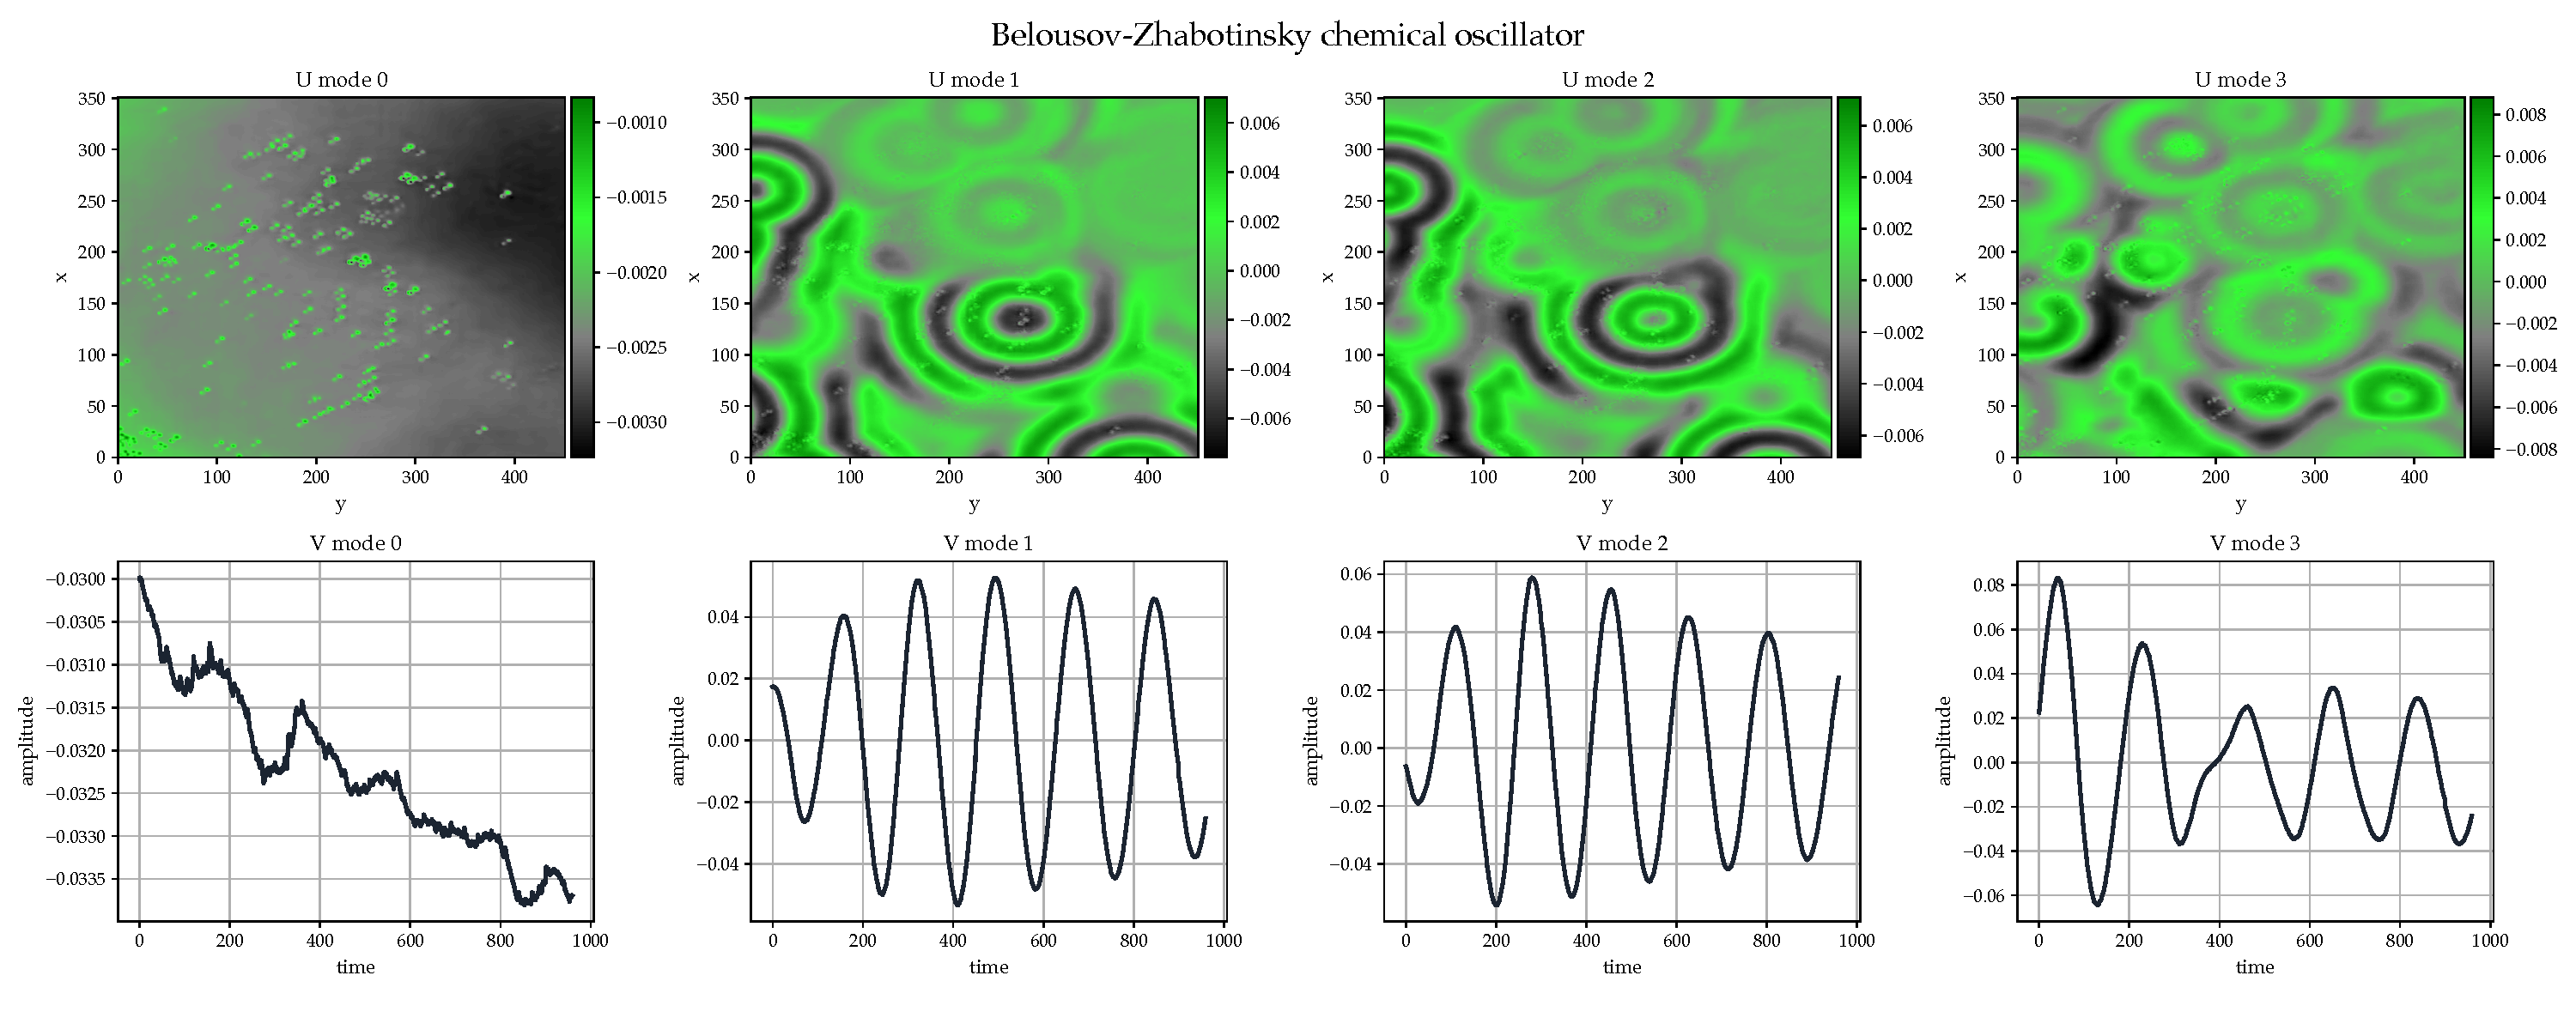
\includegraphics[width=0.9\textwidth]{../figures/BZ_firstmodes.pdf}
	\caption{First left (upper) and right (lower) singular vectors}
	\label{fig:fig16}
\end{figure}
\newpage
\section{Summary and Conclusions}
In this report, different strategies to analyze, investigate and approximate complex dynamical systems have been presented. The performance of each strategy strongly depends on the complexity of the system. Different considerations can be extracted:
\begin{itemize}
	\item SVD can be applied to reduce the dimension of the system before building complex surrogate models as a neural network.
	\item DMD can be applied to discover the principal dynamics modes and, for some problems, also to forecast the system behavior.
	\item For small-dimensional problems and small networks, the LM  algorithm allows outperforming the level of accuracy obtained with SGD.
	\item A sparse representation of the model allows gaining more insight into the behavior of the system.
	\item Its really hard to train a neural network that can be adopted as a surrogate of the Runge-Kutta scheme. One possibility to obtain better results is to combine the network with a Kalman filter or to use models that are not based on the hypothesis of a markovian process, as for example Recurrent Neural Networks (RNN).
\end{itemize}

%----------------------------------------------------------------------------------------
%	REFERENCE LIST
%----------------------------------------------------------------------------------------
\begin{thebibliography}{99} % Bibliography - this is intentionally simple in this template
	
	\bibitem[1]{brunton2019}
	Brunton, S., \& Kutz, J. (2019). Data-Driven Science and Engineering: Machine Learning, Dynamical Systems, and Control. Cambridge: Cambridge University Press.
	
	\bibitem[2]{bishop2006}
	Bishop, C.~M. (2006). Pattern Recognition and Machine Learning (Information Science and Statistics). Berlin: Springer-Verlag
	
	
\end{thebibliography}

%----------------------------------------------------------------------------------------
\appendix
\section{Codes}
All the codes have been implemented in Jupyter Notebooks. Please visit the 
\end{document}